% !TEX root = task-3-10-2.tex
% Editable task bank. Append new BankTask blocks at the end of the document.
\documentclass[12pt,a4paper]{article}
\usepackage{physics-textbook}
\usepackage{graphicx,needspace}
\usetikzlibrary{decorations.pathmorphing}
\newif\ifShowSolutions
\ifdefined\TutorEdition
  \ShowSolutionstrue
\else
  \ShowSolutionsfalse % Change to \ShowSolutionstrue to display solutions.
\fi
\newcounter{banktask}
\newsavebox{\BankTaskBox}
\newcommand{\BankTaskContent}[3]{%
  \noindent\textbf{\thebanktask.}\quad #2\par
  \ifShowSolutions
    \Needspace{50mm}% Keep the solution heading with its opening text or diagram.
    #3\par
    \ifdefined\TutorEdition
      \ifcsname TutorSource#1\endcsname
        \nopagebreak\smallskip{\small\csname TutorSource#1\endcsname\par}%
      \fi
    \fi
  \fi
}
\newcommand{\BankTask}[3]{%
  \refstepcounter{banktask}\par\medskip
  \sbox{\BankTaskBox}{\begin{minipage}{\linewidth}%
    \BankTaskContent{#1}{#2}{#3}\end{minipage}}%
  \ifdim\dimexpr\ht\BankTaskBox+\dp\BankTaskBox\relax>\dimexpr\textheight-20mm\relax
    \Needspace{35mm}\BankTaskContent{#1}{#2}{#3}%
  \else
    \Needspace{\dimexpr\ht\BankTaskBox+\dp\BankTaskBox\relax}%
    \noindent\usebox{\BankTaskBox}\par
  \fi
  \medskip
}
\begin{document}
\BookSubsection{3.10.2}{Последовательное соединение}


% Source sdamgia-2810: https://phys-ege.sdamgia.ru/problem?id=2810
\BankTask{sdamgia-2810}{
Два резистора с сопротивлениями $R_1$ и $R_2$ соединили последовательно и подключили к клеммам батарейки для карманного фонаря. Напряжение на клеммах батарейки равно $U$. Установите соответствие между физическими величинами и формулами, по которым их можно рассчитать.

\TaskMatchingColumns{Физические величины}{А) Сила тока через батарейку\par 
Б) Напряжение на резисторе с сопротивлением $R_1$}{Формулы}{$1$) $\frac{U}{R_1 + R_2}$\par 
$2$) $U ( R_1 + R_2 )$\par 
$3$) $\frac{UR_1}{R_1 + R_2}$\par 
$4$) $\frac{U}{R_1}$}

\begin{center}\small\renewcommand{\arraystretch}{1.25}\begin{tabular}{|p{0.450\linewidth}|p{0.450\linewidth}|}\hline
А & Б\\\hline
 & \\\hline
\end{tabular}\end{center}
}{
\smallskip\noindent\textbf{Решение}\par
Общее сопротивление двух последовательно соединенных резисторов с сопротивлениями $R_1$ и $R_2$ равно $R=R_1 + R_2.$ По закону Ома, сила тока через батарейку определяется выражением $I= \frac{U}{R} = \frac{U}{R_1 + R_2}$ (А — $1$). Напряжение на резисторе с сопротивлением $R_1$ равно $U_1=IR_1= \frac{U}{R_1 + R_2} R_1$ (Б — $3$).

Ответ: $13$.
}

% Source sdamgia-29117: https://phys-ege.sdamgia.ru/problem?id=29117
\BankTask{sdamgia-29117}{
Участок цепи состоит из трех последовательно соединенных резисторов с сопротивлениями $2$ Ом, $3$ Ом и $5$ Ом. Каким должно быть сопротивление четвертого резистора, который включают в этот участок последовательно к первым трем, чтобы общее сопротивление участка увеличилось в $2{,}5$ раза?

Ответ дайте в Ом.
}{
\smallskip\noindent\textbf{Решение}\par
При последовательном соединении трех сопротивлений: 

\[R_{1-3}=R_1 + R_2 + R_3=2 + 3 + 5=10\,\text{Ом}.\]

Из условия следует, что: 

\[R_{1-4}=2{,}5R_{1-3}=2{,}5 \cdot  10=25\,\text{Ом}.\]

Тогда сопротивление четвертого проводника: 

\[R_4=25 - 10=15\,\text{Ом}.\]

Ответ: $15$.
}

% Source sdamgia-29795: https://phys-ege.sdamgia.ru/problem?id=29795
\BankTask{sdamgia-29795}{
Медный цилиндрический проводник длиной $l$ подключили к источнику постоянного напряжения. При этом сила тока, текущего через проводник, равна $0{,}6$ А. Найдите силу тока, который будет течь через этот проводник, если последовательно присоединить к нему медный цилиндрический проводник длиной $2l$ того же сечения и подключить их к тому же источнику напряжения.

Ответ дайте в амперах.
}{
\smallskip\noindent\textbf{Решение}\par
Второй резистор имеет длину в $2$ раза больше. Исходя из формулы для расчета сопротивления $R= \frac{\rho l}{S} ,$ сопротивление второго проводника в $2$ раза больше, чем у первого. При последовательном соединении общее сопротивление равно сумме сопротивлений. Следовательно, общее сопротивление цепи увеличится в $3$ раза. Поскольку напряжение не изменяется, то по закону Ома для участка цепи $I= \frac{U}{R}$ сила тока уменьшится в $3$ раза и станет равной $0{,}2$ А.

Ответ: $0{,}2$.
}

% Source sdamgia-4420: https://phys-ege.sdamgia.ru/problem?id=4420
\BankTask{sdamgia-4420}{
Идеальный амперметр и три резистора сопротивлением $R=2$ Ом, $2R$ и $3R$ включены последовательно в электрическую цепь, содержащую источник с $\text{ЭДС},$ равной $5$ В, и внутренним сопротивлением $r=8$ Ом. Каковы показания амперметра? (Ответ дайте в амперах.)
}{
\smallskip\noindent\textbf{Решение}\par
Идеальный амперметр не имеет сопротивления. Согласно закону Ома для полной цепи, сила тока в описанной в условии задачи цепи (как раз то, что показывает амперметр) равна: 

\[I= \frac{\mathcal E}{r + ( R + 2R + 3R )} = \frac{\mathcal E}{r + 6R} = \frac{5\,\text{В}}{8\,\text{Ом} + 6 \cdot  2\,\text{Ом}} =0{,}25\,\text{А}.\]

Ответ: $0{,}25$.
}

% Source sdamgia-36761: https://phys-ege.sdamgia.ru/problem?id=36761
\BankTask{sdamgia-36761}{
Участок цепи состоит из двух последовательно соединенных цилиндрических проводников, сопротивление первого из которых равно $R$, а второго $2R$. Как изменится общее сопротивление этого участка цепи и тепловая мощность, выделяющаяся в первом проводнике, если удельное сопротивление и площадь поперечного сечения первого проводника увеличить вдвое, оставив без изменения его длину и напряжение на концах участка цепи? Сопротивление второго проводника не меняется.\par
$1$. Увеличится.\par
$2$. Уменьшится.\par
$3$. Не изменится.\par
\begin{center}\small\setlength{\tabcolsep}{3pt}\begin{tabular}{|p{0.45\linewidth}|p{0.45\linewidth}|}\hline
Общее сопротивление участка цепи & Тепловая мощность, выделяющаяся
в первом проводнике\\\hline
 & \\\hline
\end{tabular}\end{center}\par
}{
\smallskip\noindent\textbf{Решение}\par
А) При увеличении площади сечения и удельного сопротивления первого проводника в $2$ раза его сопротивление не изменится. Поскольку проводники соединены последовательно, то общее сопротивление участка цепи не изменится ($3$).\par
Б) Поскольку сопротивление первого проводника и напряжение не изменились, то выделяющаяся в нем тепловая мощность также не изменится ($3$).\par
Ответ: $33$.\par
}

% Source sdamgia-1428: https://phys-ege.sdamgia.ru/problem?id=1428
\BankTask{sdamgia-1428}{
Резистор $1$ с электрическим сопротивлением $3$ Ом и резистор $2$ с электрическим сопротивлением $6$ Ом включены последовательно в цепь постоянного тока. Чему равно отношение количества теплоты, выделяющегося на резисторе $1$, к количеству теплоты, выделяющемуся на резисторе $2$ за одинаковое время?
}{
\smallskip\noindent\textbf{Решение}\par
Согласно закону Джоуля — Ленца, количество теплоты, выделяющееся на проводнике при прохождении тока, пропорционально произведению квадрата силы тока, величины сопротивления проводника и времени прохождения тока: $Q=I ^2 Rt.$ Поскольку резисторы подключены последовательно, ток через них течет одинаковый, а значит, отношение количества теплоты, выделяющегося на резисторе $1$, к количеству теплоты, выделяющемуся на резисторе $2$, за одинаковое время равно: 

\[\frac{Q_1}{Q_2} = \frac{I^2R_1t}{I^2R_2t}= \frac{R_1}{R_2} = \frac{3\,\text{Ом}}{6\,\text{Ом}} =0{,}5.\]

Ответ: $0{,}5$.
}

% Source sdamgia-9741: https://phys-ege.sdamgia.ru/problem?id=9741
\BankTask{sdamgia-9741}{
Два последовательно соединенных резистора сопротивлениями $4$ Ом и $8$ Ом подключены к аккумулятору, напряжение на клеммах которого равно $24$ В. Какая тепловая мощность выделяется в резисторе большего номинала?
}{
\smallskip\noindent\textbf{Решение}\par
Резисторы подключены последовательно, а, значит, полное сопротивление цепи представляет собой сумму сопротивлений резисторов. По закону Ома в цепи течет ток, по величине равный:

$I = \frac{U}{R} = \frac{24}{4 + 8} =2$ А.

На резисторе с большим сопротивлением выделится тепловая мощность:

$P=I ^2 R=2 ^2 \cdot  8 = 32$ Вт.

Ответ: $32$.
}

% Source sdamgia-10960: https://phys-ege.sdamgia.ru/problem?id=10960
\BankTask{sdamgia-10960}{
Сопротивление одного резистора в $4$ раза больше, чем сопротивление другого. В первый раз эти резисторы соединяют параллельно, а во второй раз — последовательно. Чему равно отношение сопротивлений цепей в первом и во втором случаях?
}{
\smallskip\noindent\textbf{Решение}\par
Сопротивление участка с параллельным соединением проводов равно:

\[R_1= \frac{R \cdot  4R}{R + 4R} =0{,}8R.\]

При последовательном соединении сопротивления резисторов складываются и тогда $R_2=R + 4R=5R.$

Отношение сопротивлений цепей в первом и во втором случаях равно $\frac{R_1}{R_2} = \frac{0{,}8R}{5R} = 0{,}16.$

Ответ: $0{,}16$.
}

% Source sdamgia-25421: https://phys-ege.sdamgia.ru/problem?id=25421
\BankTask{sdamgia-25421}{
На рисунке изображена зависимость силы тока в лампе накаливания от приложенного к ней напряжения. Найдите общее напряжение на источнике тока для цепи, содержащей включенные последовательно резистор и лампу, если сила тока в цепи равна $0{,}4 \,\text{А}$, а мощность, выделяющаяся на резисторе, равна $32 \,\text{Вт}$.\par

\begin{center}\begin{tikzpicture}[book diagram,>=stealth]
\draw[task grid,step=.2](0,0)grid(4.2,2);\draw[task axis](0,0)--(4.5,0)node[right]{$U,\,\text{В}$};\draw[task axis](0,0)--(0,2.2)node[left]{$I,\,\text{А}$};\node[below left]at(0,0){$0$};\foreach\x in{40,80,120,160}\node[below]at(\x/50,0){$\x$};\foreach\y/\s in{.4/{0{,}1},.8/{0{,}2},1.2/{0{,}3},1.6/{0{,}4}}\node[left]at(0,\y){$\s$};\draw[task curve](0,0)..controls(.25,.65)and(1.5,1.26)..(2.8,1.6)..controls(3.2,1.7046153846)and(3.6,1.85)..(4,1.92);
\end{tikzpicture}\end{center}
\par
}{
\smallskip\noindent\textbf{Решение}\par
При последовательном соединении лампы и резистора сила тока через них будет одинаковой. Тогда по графику можем найти напряжение на лампе при силе тока $0{,}4 \,\text{А}$, оно равно $U_{1}\approx140\,\text{В}.$ Зная мощность тока и силу тока через резистор, найдем напряжение на нем $P_{2}=IU_{2},$ откуда $U_{2}= \frac{ P_{2}}{ I } = \frac{ 32}{ 0{,}4 } =80\,\text{В}.$ Общее напряжение при последовательном соединении равно напряжению на источнике:\par
\[U=U_{1} + U_{2}=140 + 80=220\,\text{В}.\]
Ответ: $220 \,\text{В}$.\par
}

% Source sdamgia-31898: https://phys-ege.sdamgia.ru/problem?id=31898
\BankTask{sdamgia-31898}{
Школьник заинтересовался вопросом о том, как будут светить разные лампы накаливания при различных способах их совместного использования. Для проведения опытов он взял две лампы, рассчитанные на одинаковое напряжение $220$ В. Лампа № $1$ имела номинальную мощность $40\,\text{Вт}$, а лампа № $2$ — $150\,\text{Вт}$. Сначала школьник соединил эти лампы параллельно, подключил получившуюся электрическую цепь к напряжению $127$ В и посмотрел, как светят лампы. Затем он соединил эти лампы последовательно, снова подключил получившуюся электрическую цепь к тому же напряжению $127$ В и опять посмотрел, как светят лампы.

Напишите, как светят лампы № $1$ и № $2$ при их параллельном и последовательном подключении — одинаково ярко или нет, и если не одинаково, то для каждого случая укажите, какая светит ярче.

Ответ обоснуйте, указав, какие физические закономерности Вы использовали для объяснения. Зависимость сопротивления нити лампы накаливания от температуры не учитывайте.
}{
\smallskip\noindent\textbf{Решение}\par
$1$. Если лампа рассчитана на напряжение $U=220\,\text{В}$ и имеет при этом номинальную мощность $P$, то сопротивление лампы равно $R = \frac{U ^2}{P} .$ Поэтому лампа № $1$, обладающая меньшей мощностью, имеет большее сопротивление $R_{1}$, а лампа № $2$, обладающая большей мощностью, имеет меньшее сопротивление $R_{2}$.

$2$. При параллельном подключении ламп к напряжению $U_0=127\,\text{В}$ на них падает одинаковое напряжение. Поэтому на лампе №$1$ выделяется меньшая мощность $\frac{U ^2_0}{R_1} ,$ а на лампе №$2$ — большая мощность $\frac{U ^2_0}{R_2} .$ Следовательно, лампа № $2$ в этом случае светит более ярко, чем лампа № $1$.

$3$. При последовательном подключении ламп к напряжению $U_0=127\,\text{В}$ через них протекает одинаковый ток силой: 

\[I_0 = \frac{U_0}{( R_1 + R_2 )} .\]

Поэтому на лампе № $1$ выделяется большая мощность $I ^2_0R_1,$ а на лампе №$2$ — меньшая мощность $I ^2_0R_2.$ Следовательно, лампа № $1$ в этом случае светит более ярко, чем лампа №$2$.
}


% Source 9397C7: https://ege.fipi.ru/bank/questions.php?search=1&proj=BA1F39653304A5B041B656915DC36B38&qid=9397C7
\BankTask{9397C7}{
На фотографии изображена электрическая цепь. Показания вольтметра даны в вольтах.
\par\begin{center}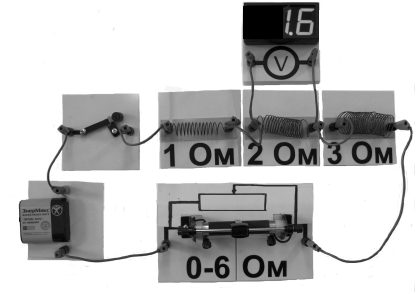
\includegraphics[width=.9\linewidth,height=.48\textheight,keepaspectratio]{_run/photos/389e5d4777aabc394c4661c2152661a8d428c2674ff93ab9ac03afcbdf49c8ea.png}\end{center}\par
Какое напряжение (в $\text{В}$) будет показывать вольтметр, если его подсоединить к резистору сопротивлением $3\,\text{Ом}$? Вольтметр считать идеальным.
}{
\smallskip\noindent\textbf{Решение от GPT}\par
На резисторе $2\,\text{Ом}$ вольтметр показывает $1{,}6\,\text{В}$. Ток в последовательно соединённых резисторах одинаков:
\[
I=\frac{1{,}6}{2}=0{,}8\,\text{А},\qquad U_3=I R_3=0{,}8\cdot3=2{,}4\,\text{В}.
\]
}

% Source DF5187: https://ege.fipi.ru/bank/questions.php?search=1&proj=BA1F39653304A5B041B656915DC36B38&qid=DF5187
\BankTask{DF5187}{
Два резистора с сопротивлениями $R_1$ и $R_2$ подключены к источнику тока с внутренним сопротивлением $r$ (см. рисунок). Напряжение на втором резисторе равно $U_2$. Чему равны напряжение на первом резисторе и ЭДС источника?

Установите соответствие между физическими величинами и формулами, по которым их можно рассчитать.

\begin{center}
\TaskMatchingColumns[0.49\linewidth]{Физические величины}{
А) напряжение на резисторе $R_1$\par
Б) ЭДС источника
}{Формулы}{
1) $\displaystyle U_2\cdot\frac{R_1}{R_2}$\par
2) $\displaystyle U_2\cdot\frac{R_2}{R_1}$\par
3) $\displaystyle\frac{U_2}{R_1}\cdot(R_1+R_2+r)$\par
4) $\displaystyle\frac{U_2}{R_2}\cdot(R_1+R_2+r)$
}

\medskip
\begin{tabular}{|c|c|}
\hline
А & Б \\
\hline
\phantom{1} & \phantom{1} \\
\hline
\end{tabular}
\end{center}

\begin{center}
\begin{tikzpicture}[book diagram,x=0.8cm,y=0.8cm]
\draw (0,1.85)--(0,3.5)--(1.4,3.5);
\draw (1.4,3.15) rectangle (3.1,3.85);
\draw (3.1,3.5)--(4.5,3.5)--(4.5,2.95);
\draw (4.15,1.25) rectangle (4.85,2.95);
\draw (4.5,1.25)--(4.5,0)--(0,0)--(0,1.55);
\draw (-0.55,1.85)--(0.55,1.85);
\draw (-0.3,1.55)--(0.3,1.55);
\node[left] at (-0.55,2.3) {$\mathcal{E},r$};
\node[below] at (2.25,3.12) {$R_1$};
\node[right] at (4.9,2.1) {$R_2$};
\end{tikzpicture}
\end{center}
}{
\smallskip\noindent\textbf{Решение от GPT}\par
При последовательном соединении ток через оба резистора одинаков: $I=U_2/R_2$. Тогда напряжение на первом резисторе $U_1=IR_1=U_2R_1/R_2$, то есть А — 1. По закону Ома для полной цепи $\mathcal{E}=I(R_1+R_2+r)=\dfrac{U_2}{R_2}(R_1+R_2+r)$, то есть Б — 4. Ответ: $14$.
}

\end{document}
